%!TEX root = ../MasterThesis.tex

\section{Computer-Supported Cooperative Work}
\label{sec:cscw}

\subsection{Fundamental aspects}
\label{sec:cscw_definition}

\gls{CSCW} is a \emph{generic} term that combines the understanding of the way people work in groups with the enabling technologies of computer networking, associated hardware, software, services and techniques. It is part of the research field of \emph{Cooperation Systems}, which emerged during the early 1980s with the understanding that a multi-disciplinary approach for \gls{IT} system design is needed for the success of such systems. As such the research field looks into the usage of applications to support group work in an organizational setting, the effects of such a system on the individual user, as well as how the applications have to be adapted for the context of the group. Therefore the studies of Cooperation Systems are consisting of a social part as well as a technical part, and are looking into the interrelationship between them for certain aspects of work in general, and explicitly for communication and cooperation in a team \citep{Grudin1994}.

% section cscw_defintion (end)

\subsection{Types of \gls{CSCW} systems}
\label{sec:cscw_types}

CSCW systems can be differentiated by their support of communication on the two axis place and time: \\

\begin{figure}[H]
 \centering
 %\includesvg[width=0.8\columnwidth, svgpath = images/]{cscw_time_place_matrix}
 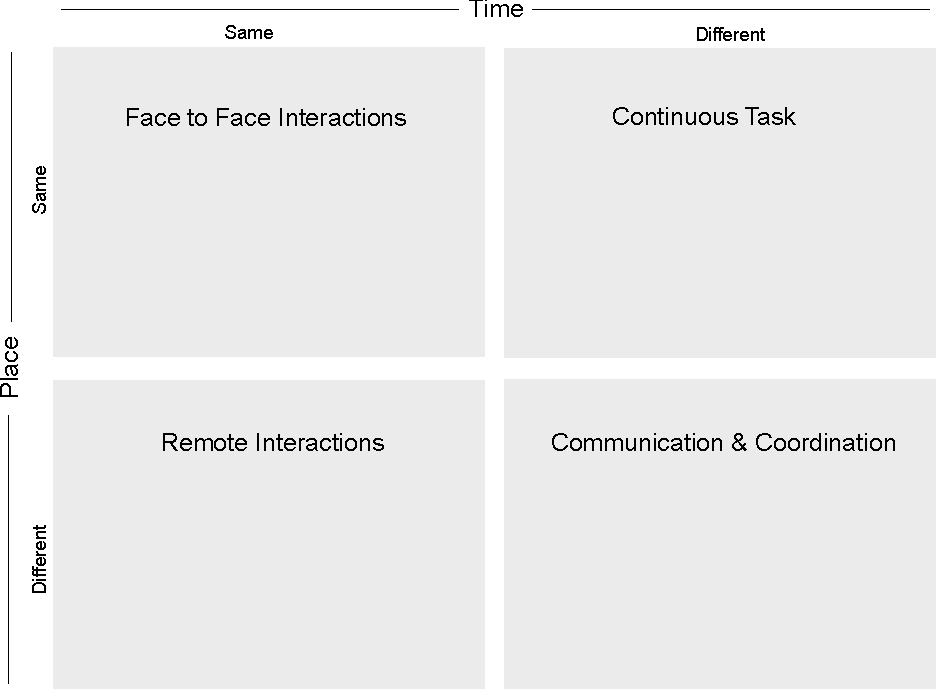
\includegraphics[width=0.8\columnwidth]{images/cscw_time_place_matrix.pdf}
 \caption[CSCW Place/Time Matrix]{\gls{CSCW} Place/Time Matrix \citep{xx}}
\label{fig:images_cscw_time_place_matrix}
\end{figure}

Additionally it is possible to group the CSCW systems based on the 3C model: \\

\begin{figure}[H]
 \centering
 %\includesvg[width=0.5\columnwidth, svgpath = images/]{cscw_time_place_matrix}
 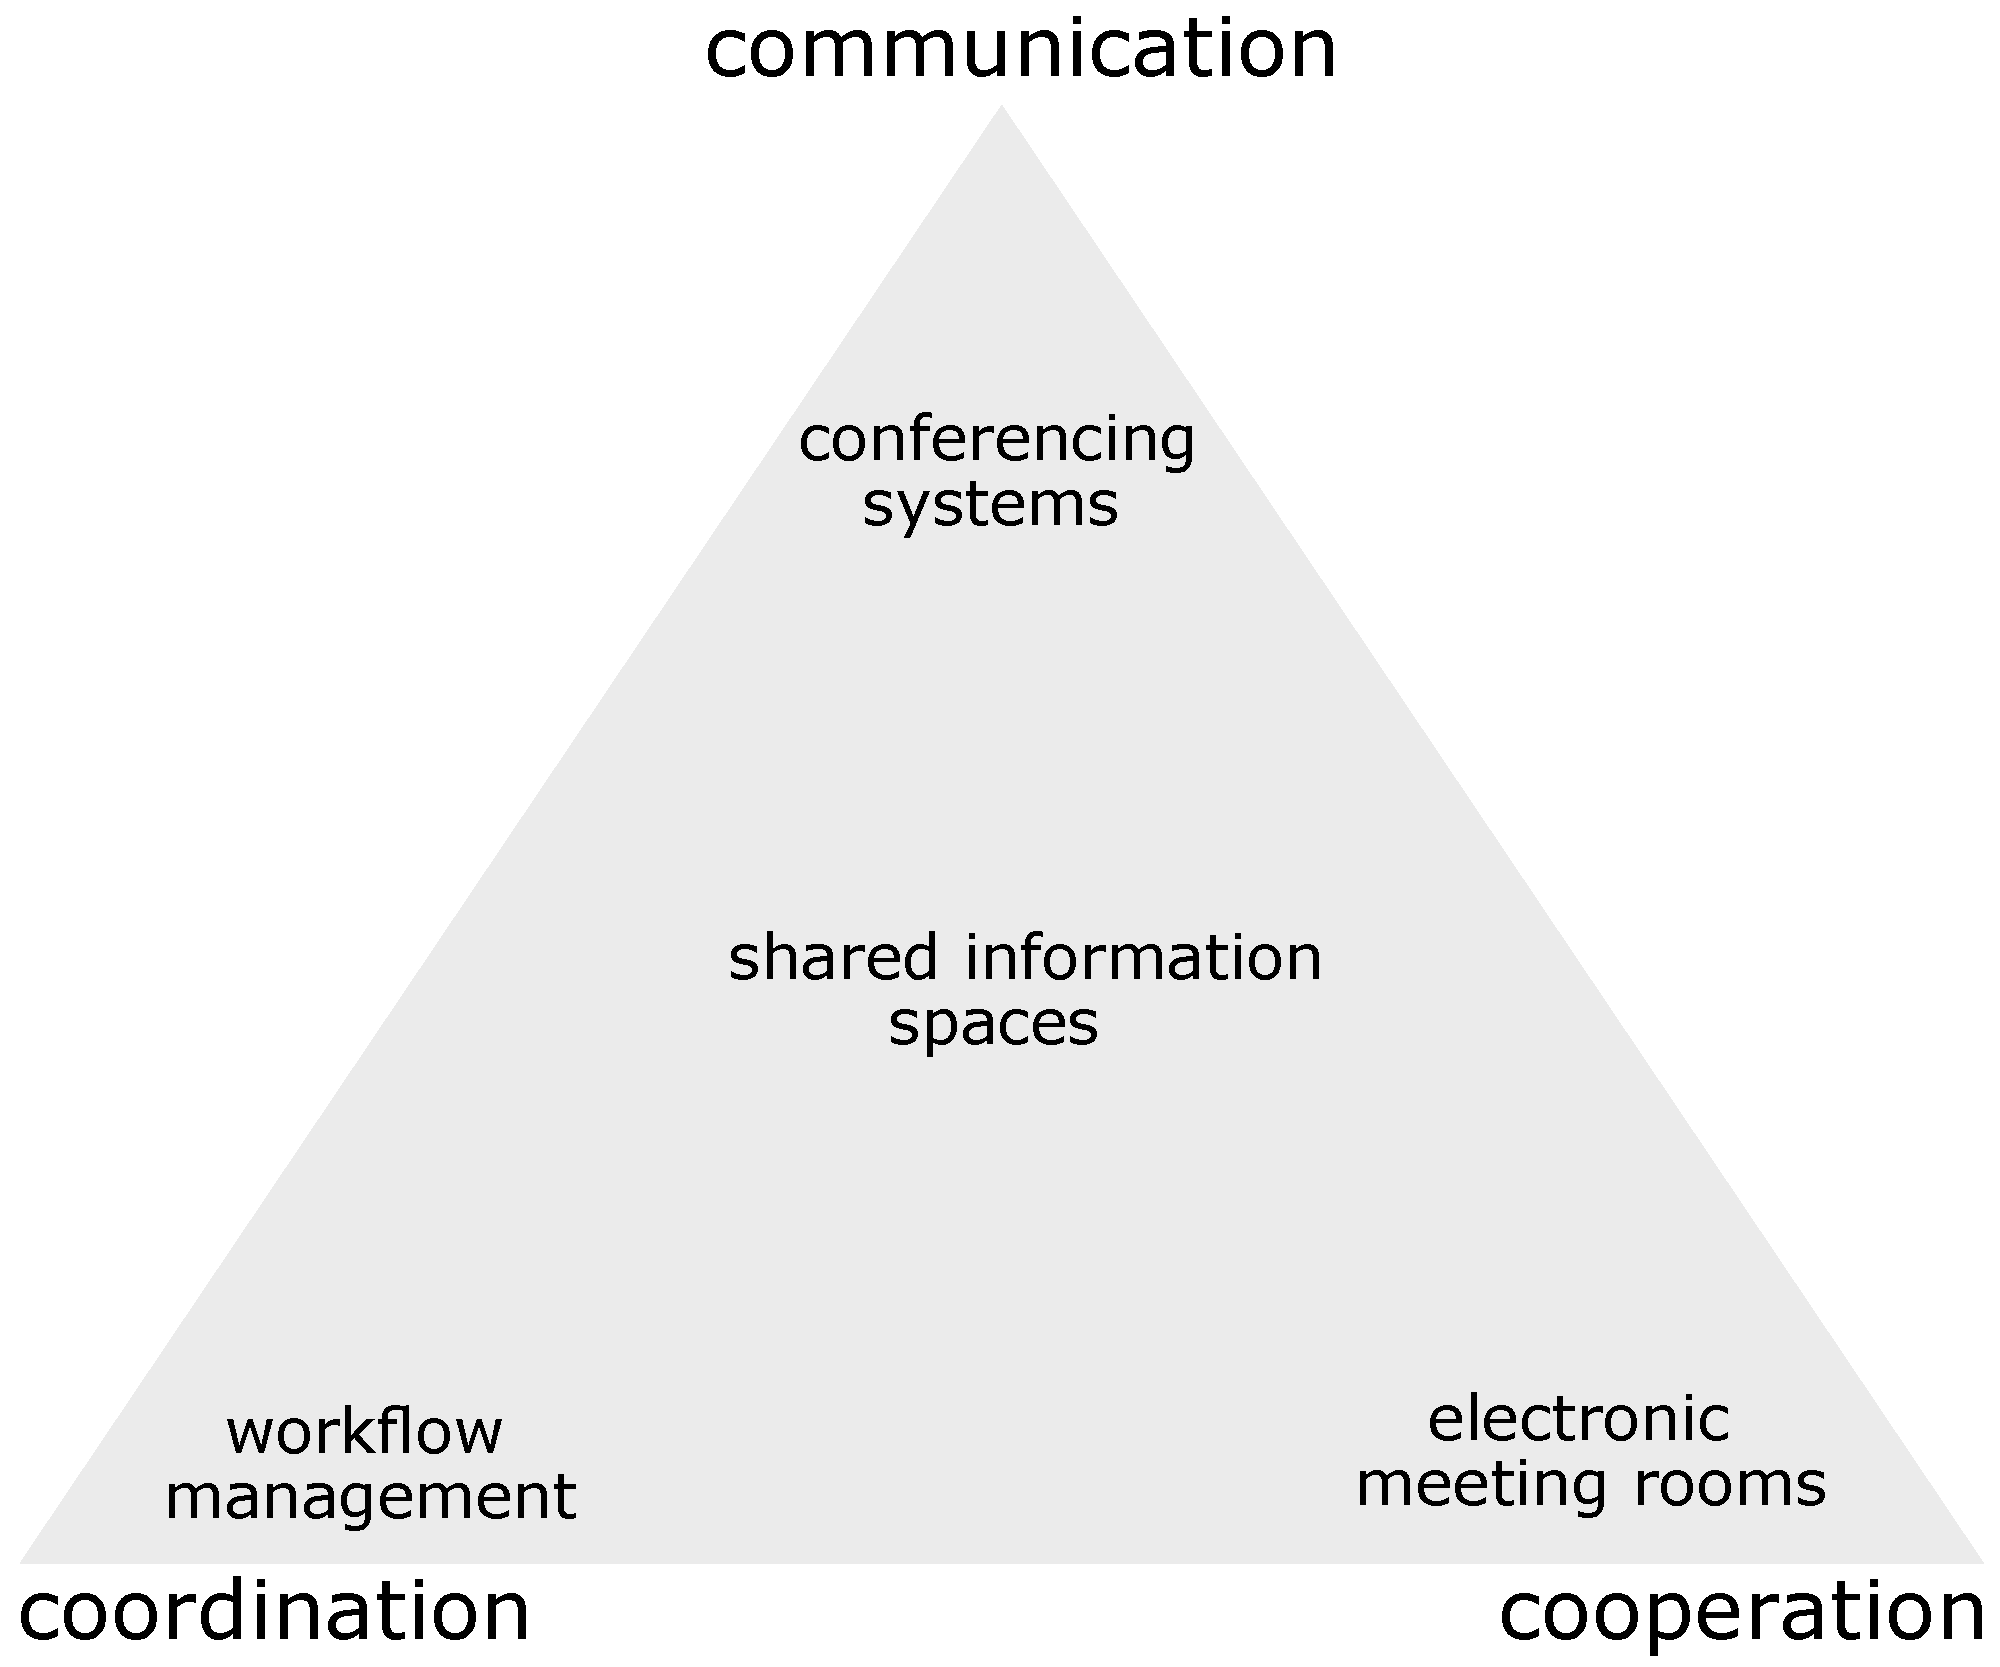
\includegraphics[width=0.8\columnwidth]{images/3C-model.pdf}
 \caption[The 3C Model]{The 3C Model \citep{Koch2008}}
\label{fig:images_cscw_3C_model}
\end{figure}

% section cscw_types (end)

\subsection{Shared Information Spaces}
\label{sec:cscw_shared_spaces}

% section cscw_shared_spaces (end)

% section cscw (end)
